\section{What is Survival Analysis?}

Survival analysis comprises a collection of statistical methods designed for analyzing \textbf{time-to-event data} - data where the primary interest is in the time until a specific event occurs. Unlike standard regression or classification problems, survival analysis specifically addresses scenarios where we want to answer "how long until" questions. These methods have widespread applications across multiple disciplines:

\begin{itemize}
    \item \textbf{Medical research:} How long will a patient survive following diagnosis? What factors affect progression-free survival?
    \item \textbf{Engineering:} When will a machine component fail? How does maintenance affect lifetime?
    \item \textbf{Economics:} How long will a customer maintain a subscription? What influences customer retention?
    \item \textbf{Sociology:} When will someone find employment after completing education? What factors affect time to re-employment?
\end{itemize}

\begin{notebox}[title=Key Terminology]
Different fields often use different terminology for the same survival analysis concepts:
\begin{itemize}
    \item \textbf{Medicine:} Survival analysis, time-to-event analysis
    \item \textbf{Engineering:} Reliability analysis, failure time analysis
    \item \textbf{Economics:} Duration analysis, event history analysis
    \item \textbf{Sociology:} Event history analysis, transition analysis
\end{itemize}
Despite these different names, the underlying statistical principles remain the same.
\end{notebox}

\section{Distinctive Features of Survival Data}

Survival data possesses several unique characteristics that distinguish it from other types of data and necessitate specialized analytical methods:

\subsection{Censoring}

The most distinctive feature of survival data is \textbf{censoring}, which occurs when we do not observe the exact time of the event for some subjects. Censoring introduces a fundamental challenge: we have incomplete information, but that incomplete information still provides valuable insights that we need to incorporate into our analysis.

\begin{definitionbox}[title=Censoring]
Censoring occurs when the event of interest is not observed within the study period or observation window. Instead of the exact event time, we only know that the event either:
\begin{itemize}
    \item Has not yet occurred by a certain time (right censoring)
    \item Occurred before a certain time (left censoring)
    \item Occurred within a specific time interval (interval censoring)
\end{itemize}
\end{definitionbox}

\subsubsection{Right Censoring}

Right censoring is the most common type of censoring in survival analysis. It occurs when a subject exits the study before experiencing the event of interest.

\begin{examplebox}[title=Examples of Right Censoring]
\begin{itemize}
    \item A patient is still alive at the end of a clinical trial's follow-up period
    \item A study participant withdraws from the study before experiencing the event
    \item A customer is still subscribed to a service when data collection ends
    \item A machine component is still functioning at the end of an observation period
\end{itemize}

In each case, we only know that the subject survived \textit{at least} until the censoring time, but we don't know the exact event time.
\end{examplebox}

Figure \ref{fig:right-censoring} illustrates right censoring in a hypothetical clinical study. Subjects 1 and 2 experience the event of interest (e.g., disease progression), while Subject 3 is right-censored at the end of the study period.

\begin{figure}[htbp]
    \centering
    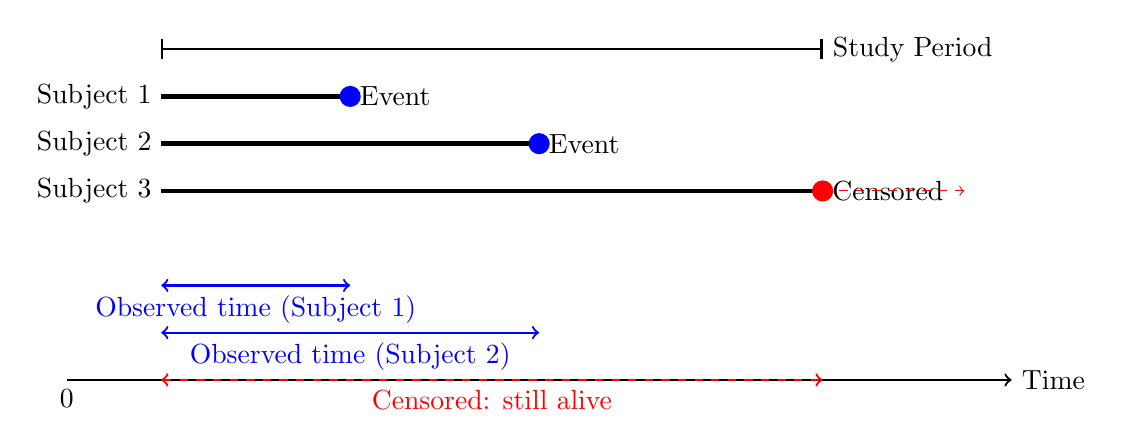
\begin{tikzpicture}[scale=1.2]
        % Timeline
        \draw[->, thick] (0,0) -- (10,0) node[right] {Time};
        \draw (0,0) node[below] {0};

        % Study period
        \draw[|-|, thick] (1,3.5) -- (8,3.5) node[right] {Study Period};

        % Subject 1: Experiences event
        \draw[ultra thick, -] (1,3) -- (3,3);
        \filldraw[blue] (3,3) circle (3pt);
        \node[left] at (1,3) {Subject 1};
        \node[right] at (3,3) {Event};

        % Subject 2: Experiences event
        \draw[ultra thick, -] (1,2.5) -- (5,2.5);
        \filldraw[blue] (5,2.5) circle (3pt);
        \node[left] at (1,2.5) {Subject 2};
        \node[right] at (5,2.5) {Event};

        % Subject 3: Right censored
        \draw[ultra thick, -] (1,2) -- (8,2);
        \filldraw[red] (8,2) circle (3pt);
        \node[left] at (1,2) {Subject 3};
        \node[right] at (8,2) {Censored};
        \draw[red, dashed, ->] (8,2) -- (9.5,2);

        % Observation periods
        \draw[<->, thick, blue] (1,1) -- (3,1) node[midway, below] {Observed time (Subject 1)};
        \draw[<->, thick, blue] (1,0.5) -- (5,0.5) node[midway, below] {Observed time (Subject 2)};
        \draw[<->, thick, red, dashed] (1,0) -- (8,0) node[midway, below] {Censored: still alive};
    \end{tikzpicture}
    \caption{Illustration of right censoring in a clinical study. Subjects 1 and 2 experience the event of interest, while Subject 3 is right-censored at the end of the study period. We know Subject 3 survived at least until time 8, but we don't know their exact event time.}
    \label{fig:right-censoring}
\end{figure}

\subsubsection{Left Censoring}

Left censoring occurs when the event of interest happens before the first observation time, but we don't know exactly when it occurred.

\begin{examplebox}[title=Examples of Left Censoring]
\begin{itemize}
    \item A patient already has the disease when first examined, but we don't know when it developed
    \item Environmental contamination detected at the start of monitoring, but we don't know when it began
    \item A customer had already canceled their subscription before the study began
    \item A component is discovered to be already failed at the first inspection
\end{itemize}

In these cases, we only know that the event occurred \textit{sometime before} the first observation.
\end{examplebox}

Figure \ref{fig:left-censoring} shows left censoring in a disease monitoring study. Subject 1 is found to have the disease at the study entry, representing left censoring.

\begin{figure}[htbp]
    \centering
    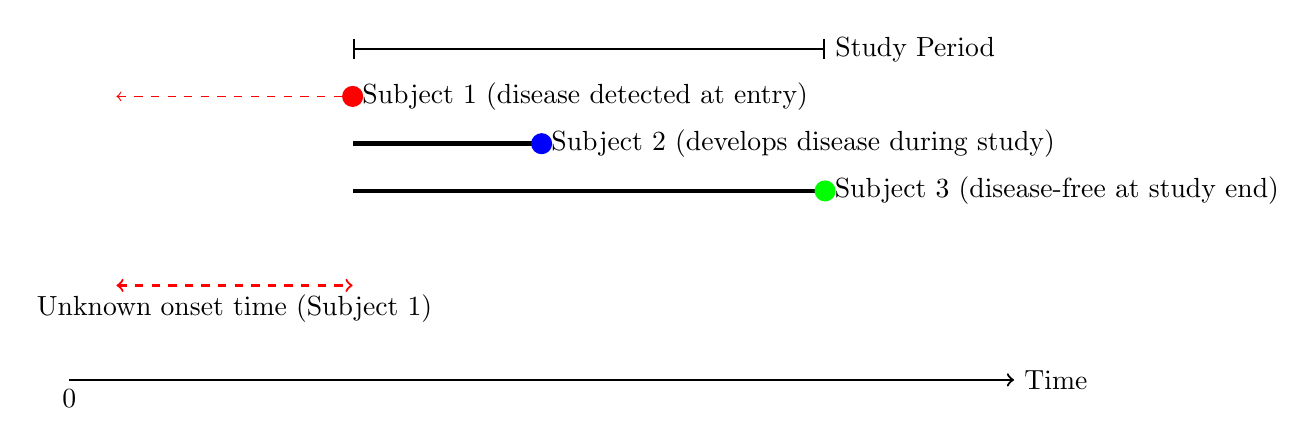
\begin{tikzpicture}[scale=1.2]
        % Timeline
        \draw[->, thick] (0,0) -- (10,0) node[right] {Time};
        \draw (0,0) node[below] {0};

        % Study period
        \draw[|-|, thick] (3,3.5) -- (8,3.5) node[right] {Study Period};

        % Subject 1: Left censored
        \filldraw[red] (3,3) circle (3pt);
        \draw[red, dashed, <-] (0.5,3) -- (3,3);
        \node[right] at (3,3) {Subject 1 (disease detected at entry)};

        % Subject 2: Experiences event
        \draw[ultra thick, -] (3,2.5) -- (5,2.5);
        \filldraw[blue] (5,2.5) circle (3pt);
        \node[right] at (5,2.5) {Subject 2 (develops disease during study)};

        % Subject 3: Right censored
        \draw[ultra thick, -] (3,2) -- (8,2);
        \filldraw[green] (8,2) circle (3pt);
        \node[right] at (8,2) {Subject 3 (disease-free at study end)};

        % Observation arrows
        \draw[<->, thick, red, dashed] (0.5,1) -- (3,1);
        \node[below] at (1.75,1) {Unknown onset time (Subject 1)};
    \end{tikzpicture}
    \caption{Illustration of left censoring. Subject 1 already has the disease when entering the study, so we only know the disease onset occurred sometime before the study entry point.}
    \label{fig:left-censoring}
\end{figure}

\subsubsection{Interval Censoring}

Interval censoring occurs when we know the event occurred within a specific time interval, but not the exact time.

\begin{examplebox}[title=Examples of Interval Censoring]
\begin{itemize}
    \item A tumor is detected during a regular screening visit, but was not present at the previous visit
    \item Infection is detected during a follow-up visit, but was not present at the previous visit
    \item A machine is found to be malfunctioning during a scheduled inspection, but was working at the last inspection
    \item A crack in a structure is discovered during routine examination, but was not present at the previous examination
\end{itemize}

We know the event occurred within the interval between observations, but not the exact time.
\end{examplebox}

Figure \ref{fig:interval-censoring} illustrates interval censoring in a periodic screening context. The condition is detected at Visit 3, but was not present at Visit 2, so the exact onset time is interval-censored between these visits.

\begin{figure}[htbp]
    \centering
    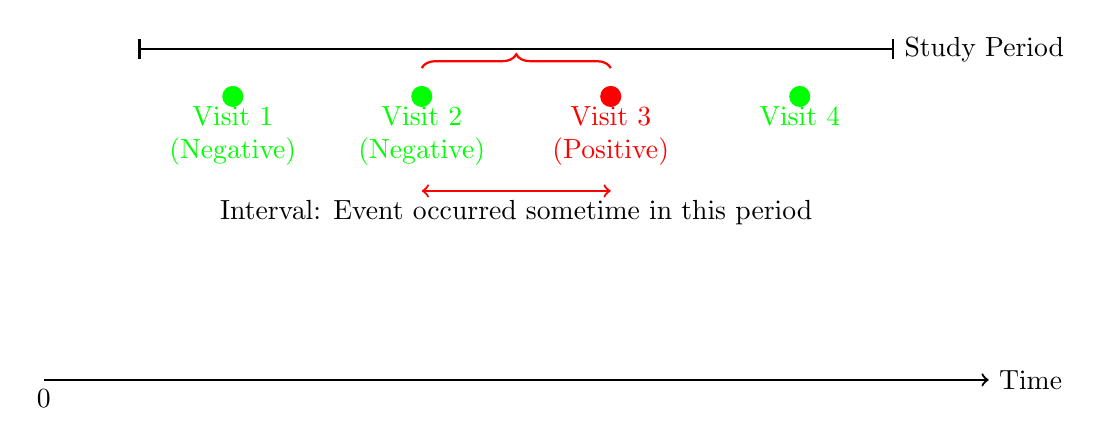
\begin{tikzpicture}[scale=1.2]
        % Timeline
        \draw[->, thick] (0,0) -- (10,0) node[right] {Time};
        \draw (0,0) node[below] {0};

        % Study period
        \draw[|-|, thick] (1,3.5) -- (9,3.5) node[right] {Study Period};

        % Checkup times
        \filldraw[green] (2,3) circle (3pt) node[below, align=center] {Visit 1\\(Negative)};
        \filldraw[green] (4,3) circle (3pt) node[below, align=center] {Visit 2\\(Negative)};
        \filldraw[red] (6,3) circle (3pt) node[below, align=center] {Visit 3\\(Positive)};
        \filldraw[green] (8,3) circle (3pt) node[below] {Visit 4};

        % Interval censoring
        \draw[<->, thick, red] (4,2) -- (6,2);
        \node[below] at (5,2) {Interval: Event occurred sometime in this period};

        % Highlight interval
        \draw[red, thick, decorate, decoration={brace, amplitude=5pt}] (4,3.3) -- (6,3.3);
    \end{tikzpicture}
    \caption{Illustration of interval censoring. The condition is negative at Visit 2 but positive at Visit 3, so we know the onset occurred within this time interval, but not the exact time.}
    \label{fig:interval-censoring}
\end{figure}

\subsection{Time-Varying Effects and Covariates}

In survival analysis, the relationship between predictors and outcomes can change over time:

\begin{itemize}
    \item \textbf{Time-varying effects:} The impact of a covariate on survival may change over time. For example, a treatment might be most effective in the short term but diminish in effectiveness over time.

    \item \textbf{Time-varying covariates:} The values of predictors may change over the course of observation. For instance, a patient's biomarker levels or medication dosages might change throughout a study.
\end{itemize}

\subsection{Multiple Outcomes and Competing Risks}

In many real-world scenarios, subjects may experience different types of events:

\begin{itemize}
    \item \textbf{Competing risks:} Multiple possible event types where the occurrence of one event precludes the observation of others. For example, patients might die from cancer, heart disease, or other causes, but once one cause of death occurs, the others cannot be observed.

    \item \textbf{Recurrent events:} The same event can occur multiple times for a subject, such as hospital readmissions or equipment failures.

    \item \textbf{Multi-state processes:} Subjects can transition through various states over time, like different stages of disease progression.
\end{itemize}

\section{Core Questions in Survival Analysis}

Survival analysis addresses several fundamental questions:

\subsection{Survival Probability Estimation}

What is the probability that a subject will survive (not experience the event) beyond a specific time point? This is typically represented by the \textit{survival function}, denoted as $S(t)$, which gives the probability of surviving beyond time $t$.

\begin{equationbox}[title=Survival Function]
\begin{equation}
S(t) = P(T > t)
\end{equation}

where $T$ is the time-to-event random variable. The survival function has the following properties:
\begin{itemize}
    \item $S(0) = 1$ (all subjects are event-free at the start)
    \item $\lim_{t \to \infty} S(t) = 0$ (eventually all subjects experience the event)
    \item $S(t)$ is monotonically decreasing (survival probability cannot increase with time)
\end{itemize}
\end{equationbox}

Figure \ref{fig:survival-function} shows a typical survival curve, which illustrates how the probability of surviving beyond time $t$ decreases over time.

\begin{figure}[htbp]
    \centering
    \begin{tikzpicture}
        \begin{axis}[
            width=0.8\textwidth,
            height=6cm,
            xlabel={Time},
            ylabel={$S(t)$},
            axis lines=left,
            xmin=0, xmax=10,
            ymin=0, ymax=1.05,
            domain=0:10,
            samples=100
        ]
            % Example survival function
            \addplot[blue, thick] {exp(-0.2*x)};

            % Annotation for specific S(t) value
            \addplot[gray, dashed, samples=2] coordinates {(3,0) (3,0.55)};
            \draw[<->] (axis cs:3.2,0) -- (axis cs:3.2,0.55) node[midway, right] {$S(3) = 0.55$};

            % Median survival
            \addplot[gray, dashed, samples=2] coordinates {(0,0.5) (10,0.5)};
            \addplot[gray, dashed, samples=2] coordinates {(3.47,0) (3.47,0.5)};
            \node[below] at (axis cs:3.47,0) {Median survival};
        \end{axis}
    \end{tikzpicture}
    \caption{A typical survival function showing the probability of surviving beyond time $t$. The dashed lines indicate how to find the median survival time (where $S(t) = 0.5$).}
    \label{fig:survival-function}
\end{figure}

\subsection{Risk Assessment: Hazard Function}

What is the instantaneous risk of experiencing the event at a specific time, given survival up to that time? This is represented by the \textit{hazard function}, denoted as $h(t)$.

\begin{equationbox}[title=Hazard Function]
\begin{equation}
h(t) = \lim_{\Delta t \to 0} \frac{P(t \leq T < t + \Delta t | T \geq t)}{\Delta t}
\end{equation}

The hazard function represents the instantaneous rate of event occurrence at time $t$, conditional on having survived until time $t$.
\end{equationbox}

Unlike the survival function, the hazard function can take many shapes, as illustrated in Figure \ref{fig:hazard-patterns}.

\begin{figure}[htbp]
    \centering
    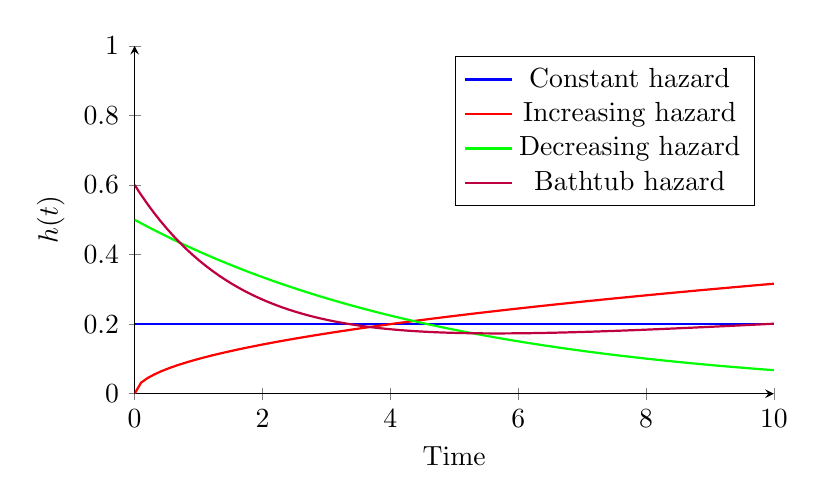
\begin{tikzpicture}
        \begin{axis}[
            width=0.8\textwidth,
            height=6cm,
            xlabel={Time},
            ylabel={$h(t)$},
            axis lines=left,
            xmin=0, xmax=10,
            ymin=0, ymax=1,
            domain=0:10,
            samples=100,
            legend pos=north east
        ]
            % Constant hazard (Exponential distribution)
            \addplot[blue, thick] {0.2};
            \addlegendentry{Constant hazard};

            % Increasing hazard (Weibull with shape > 1)
            \addplot[red, thick] {0.1*x^0.5};
            \addlegendentry{Increasing hazard};

            % Decreasing hazard (Weibull with shape < 1)
            \addplot[green, thick] {0.5*exp(-0.2*x)};
            \addlegendentry{Decreasing hazard};

            % Bathtub hazard (common in reliability)
            \addplot[purple, thick] {0.5*exp(-0.6*x) + 0.1 + 0.01*x};
            \addlegendentry{Bathtub hazard};
        \end{axis}
    \end{tikzpicture}
    \caption{Different patterns of hazard functions. The constant hazard corresponds to the exponential distribution, increasing hazard might indicate aging or wear, decreasing hazard can represent early failures, and the bathtub pattern is common in reliability engineering.}
    \label{fig:hazard-patterns}
\end{figure}

\subsection{Covariate Effects}

How do various factors (covariates) affect survival probabilities and hazard rates? This is typically addressed through regression models that relate covariates to the hazard function or survival function.

\begin{equationbox}[title=Cox Proportional Hazards Model]
\begin{equation}
h(t|\mathbf{X}) = h_0(t) \exp(\boldsymbol{\beta}^T \mathbf{X})
\end{equation}

where $h_0(t)$ is the baseline hazard function, $\mathbf{X}$ is the vector of covariates, and $\boldsymbol{\beta}$ represents the coefficients indicating how each covariate affects the hazard ratio.
\end{equationbox}

\subsection{Group Comparisons}

Are there differences in survival experiences between groups? This is often assessed using non-parametric tests like the log-rank test or through regression modeling.

\subsection{Advanced Questions}

As the field progresses, particularly with the incorporation of machine learning techniques, additional questions are being addressed:

\begin{itemize}
    \item How to model complex, non-linear relationships between covariates and outcomes?
    \item How to incorporate unstructured data (images, text, etc.) into survival models?
    \item How to handle competing risks and multi-state processes efficiently?
    \item How to provide uncertainty quantification for survival predictions?
    \item How to use survival predictions to guide personalized treatment decisions?
\end{itemize}

\section{Traditional Approaches to Survival Analysis}

Survival analysis has traditionally been approached through three main categories of methods: non-parametric, semi-parametric, and fully parametric. Each has its strengths and limitations.

\subsection{Non-Parametric Methods}

Non-parametric methods make no assumptions about the underlying distribution of survival times. They are useful for exploratory analysis and for comparing survival experiences between groups.

\subsubsection{Kaplan-Meier Estimator}

The Kaplan-Meier estimator is the most widely used non-parametric method for estimating the survival function from censored data.

\begin{equationbox}[title=Kaplan-Meier Estimator]
\begin{equation}
\hat{S}(t) = \prod_{t_i \leq t} \left(1 - \frac{d_i}{n_i}\right)
\end{equation}

where:
\begin{itemize}
    \item $t_i$ are the distinct event times observed in the data
    \item $d_i$ is the number of events at time $t_i$
    \item $n_i$ is the number of subjects at risk just before time $t_i$
\end{itemize}
\end{equationbox}

The Kaplan-Meier estimator produces a step function that decreases at each event time, as shown in Figure \ref{fig:kaplan-meier}.

\begin{figure}[htbp]
    \centering
    \begin{tikzpicture}
        \begin{axis}[
            width=0.8\textwidth,
            height=6cm,
            xlabel={Time},
            ylabel={$\hat{S}(t)$},
            axis lines=left,
            ymin=0, ymax=1.05,
            xmin=0, xmax=10,
            xtick={0,2,...,10},
            ytick={0,0.2,...,1},
            domain=0:10,
            samples=100
        ]
            % Step function
            \addplot[blue, thick, const plot, jump mark left] coordinates {
                (0,1) (1,1) (1,0.9)
                (2,0.9) (2,0.8) (3,0.8)
                (3,0.7) (4,0.7) (4,0.6)
                (5,0.6) (5,0.5) (6,0.5)
                (6,0.4) (7,0.4) (7,0.3)
                (8,0.3) (8,0.2) (9,0.2)
                (9,0.1) (10,0.1)
            };

            % Censored points (open circles)
            \addplot[
                only marks,
                mark=o,
                mark options={fill=white, draw=black},
                mark size=2.5pt
            ] coordinates {
                (1.5,0.9)
                (3.5,0.7)
                (6.5,0.4)
                (9.5,0.1)
            };

            % Event markers (filled circles)
            \addplot[
                only marks,
                mark=*,
                color=blue,
                mark size=2pt
            ] coordinates {
                (1,0.9)
                (2,0.8)
                (3,0.7)
                (4,0.6)
                (5,0.5)
                (6,0.4)
                (7,0.3)
                (8,0.2)
                (9,0.1)
            };

            % Median survival
            \addplot[gray, dashed, samples=2] coordinates {(0,0.5) (10,0.5)};
            \addplot[gray, dashed, samples=2] coordinates {(5,0) (5,0.5)};
        \end{axis}
    \end{tikzpicture}
    \caption{Kaplan-Meier survival curve. The step function drops at each event time, and censored observations are shown as open circles. The median survival time is 5 (where the curve crosses the 0.5 probability line).}
    \label{fig:kaplan-meier}
\end{figure}

\subsubsection{Log-Rank Test}

The Log-Rank test is a non-parametric statistical test used to compare survival distributions between two or more groups.

\begin{equationbox}[title=Log-Rank Test Statistic]
\begin{equation}
\chi^2 = \frac{(O_1 - E_1)^2}{E_1} + \frac{(O_2 - E_2)^2}{E_2} + \cdots + \frac{(O_G - E_G)^2}{E_G}
\end{equation}

where:
\begin{itemize}
    \item $O_g$ is the observed number of events in group $g$
    \item $E_g$ is the expected number of events in group $g$ under the null hypothesis
    \item $G$ is the number of groups
\end{itemize}
The test statistic follows a chi-square distribution with $(G-1)$ degrees of freedom under the null hypothesis of no difference between groups.
\end{equationbox}

\subsection{Semi-Parametric Methods}

Semi-parametric methods make some assumptions about the relationship between covariates and hazard, but leave the baseline hazard function unspecified.

\subsubsection{Cox Proportional Hazards Model}

The Cox proportional hazards model is the most widely used regression model in survival analysis. It assumes that the effect of covariates is to multiply the hazard by a constant factor, but makes no assumptions about the shape of the baseline hazard.

\begin{equationbox}[title=Cox Proportional Hazards Model]
\begin{equation}
h(t|\mathbf{X}) = h_0(t) \exp(\boldsymbol{\beta}^T \mathbf{X})
\end{equation}

where:
\begin{itemize}
    \item $h_0(t)$ is the baseline hazard function (left unspecified)
    \item $\mathbf{X}$ is the vector of covariates
    \item $\boldsymbol{\beta}$ is the vector of regression coefficients
\end{itemize}

The key assumption is that the hazard ratio between any two individuals is constant over time (proportional hazards assumption).
\end{equationbox}

The Cox model can be fit using partial likelihood, which allows estimation of $\boldsymbol{\beta}$ without having to specify $h_0(t)$. This makes it very flexible and robust.

\begin{figure}[htbp]
    \centering
    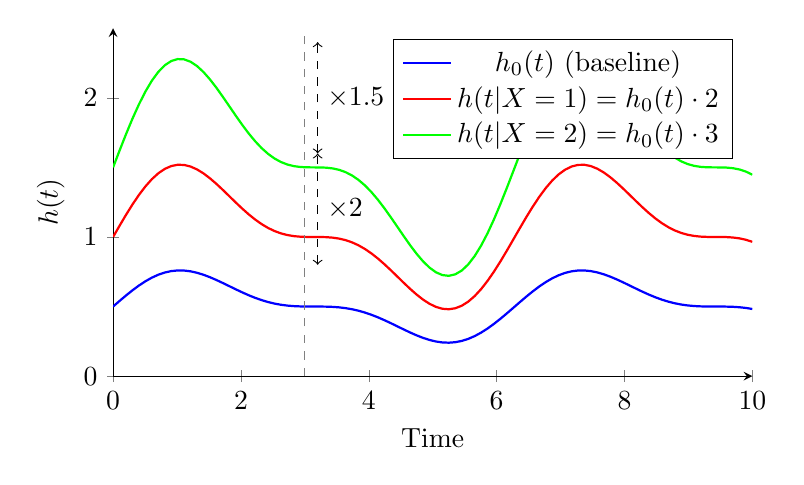
\begin{tikzpicture}
        \begin{axis}[
            width=0.8\textwidth,
            height=6cm,
            xlabel={Time},
            ylabel={$h(t)$},
            axis lines=left,
            ymin=0, ymax=2.5,
            xmin=0, xmax=10,
            domain=0:10,
            samples=100,
            legend pos=north east
        ]
            % Baseline hazard
            \addplot[blue, thick] {0.5 + 0.2*sin(deg(x)) + 0.1*sin(deg(2*x))};
            \addlegendentry{$h_0(t)$ (baseline)};

            % Proportional hazard for X=1
            \addplot[red, thick] {2*(0.5 + 0.2*sin(deg(x)) + 0.1*sin(deg(2*x)))};
            \addlegendentry{$h(t|X=1) = h_0(t) \cdot 2$};

            % Proportional hazard for X=2
            \addplot[green, thick] {3*(0.5 + 0.2*sin(deg(x)) + 0.1*sin(deg(2*x)))};
            \addlegendentry{$h(t|X=2) = h_0(t) \cdot 3$};

            % Vertical reference line
            \addplot[gray, dashed, samples=2] coordinates {(3,0) (3,2.5)};

            % Proportional hazards illustration
            \draw[<->, dashed] (axis cs:3.2,0.8) -- (axis cs:3.2,1.6) node[midway, right] {$\times 2$};
            \draw[<->, dashed] (axis cs:3.2,1.6) -- (axis cs:3.2,2.4) node[midway, right] {$\times 1.5$};
        \end{axis}
    \end{tikzpicture}
    \caption{Illustration of the proportional hazards assumption in the Cox model. The hazard ratios between different covariate values remain constant over time, regardless of the shape of the baseline hazard.}
    \label{fig:proportional-hazards}
\end{figure}

\subsubsection{Extensions of the Cox Model}

Several extensions of the Cox model have been developed to address specific limitations:

\begin{itemize}
    \item \textbf{Stratified Cox model:} Allows for different baseline hazards across strata while maintaining the same covariate effects.

    \item \textbf{Time-dependent Cox model:} Allows for time-varying covariates and time-varying effects through terms like $X(t)$ and $\beta(t)$.

    \item \textbf{Frailty models:} Incorporate random effects to account for unobserved heterogeneity and clustering in the data.

    \item \textbf{Competing risks extensions:} Adaptations for handling competing events, such as cause-specific Cox models and Fine-Gray models.
\end{itemize}

\subsection{Fully Parametric Methods}

Parametric methods specify a full probability distribution for the survival times. These methods are more efficient when the distributional assumptions are correct and allow for direct modeling of the survival time rather than just the hazard.

\subsubsection{Common Parametric Distributions}

Several probability distributions are commonly used in parametric survival analysis:

\paragraph{Exponential Distribution}
The exponential distribution assumes a constant hazard rate, which corresponds to a memoryless process.

\begin{equationbox}[title=Exponential Distribution]
\begin{align}
h(t) &= \lambda\\
S(t) &= e^{-\lambda t}\\
f(t) &= \lambda e^{-\lambda t}
\end{align}

where $\lambda > 0$ is the rate parameter.
\end{equationbox}

\paragraph{Weibull Distribution}
The Weibull distribution allows for both increasing and decreasing hazard rates, depending on the shape parameter.

\begin{equationbox}[title=Weibull Distribution]
\begin{align}
h(t) &= \alpha \lambda (\lambda t)^{\alpha-1}\\
S(t) &= e^{-(\lambda t)^\alpha}\\
f(t) &= \alpha \lambda (\lambda t)^{\alpha-1} e^{-(\lambda t)^\alpha}
\end{align}

where $\alpha > 0$ is the shape parameter and $\lambda > 0$ is the scale parameter.
\begin{itemize}
    \item If $\alpha = 1$, the Weibull reduces to the exponential distribution
    \item If $\alpha > 1$, the hazard increases with time
    \item If $\alpha < 1$, the hazard decreases with time
\end{itemize}
\end{equationbox}

\paragraph{Log-normal and Log-logistic Distributions}
These distributions can model non-monotonic hazard rates, where the hazard first increases and then decreases over time.

\paragraph{Generalized Gamma Distribution}
A flexible three-parameter family that includes many other distributions as special cases.

\begin{figure}[htbp]
    \centering
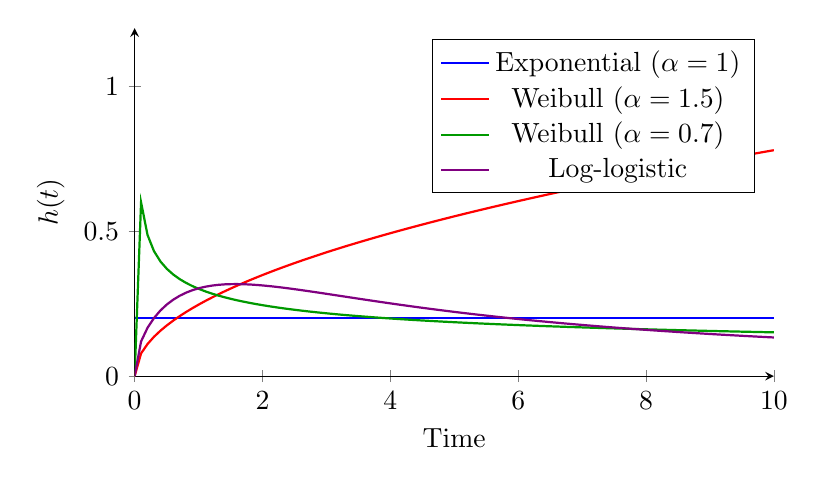
\begin{tikzpicture}
    \begin{axis}[
        width=0.8\textwidth,
        height=6cm,
        xlabel={Time},
        ylabel={$h(t)$},
        axis lines=left,
        ymin=0, ymax=1.2,
        xmin=0, xmax=10,
        domain=0:10,
        samples=100,
        legend pos=north east
    ]
        % Exponential hazard (constant)
        \addplot[blue, thick] {0.2};
        \addlegendentry{Exponential ($\alpha=1$)};

        % Weibull increasing
        \addplot[red, thick] {0.45 * pow(0.3*x, 0.5)};
        \addlegendentry{Weibull ($\alpha=1.5$)};

        % Weibull decreasing
        \addplot[green!60!black, thick] {0.21 * pow(0.3*x, -0.3)};
        \addlegendentry{Weibull ($\alpha=0.7$)};

        % Log-logistic (non-monotonic)
        \addplot[violet, thick] {0.6 * pow(0.4*x, 0.5) / (1 + pow(0.4*x, 1.5))};
        \addlegendentry{Log-logistic};
    \end{axis}
\end{tikzpicture}
    \caption{Hazard functions for different parametric survival distributions. Note how the shape parameter in the Weibull distribution controls whether the hazard increases or decreases with time, while the log-logistic allows for a non-monotonic hazard.}
    \label{fig:parametric-hazards}
\end{figure}

\subsubsection{Parametric Regression Models}

Parametric regression models relate covariates to the parameters of these distributions. For example, in a Weibull regression model:

\begin{equationbox}[title=Parametric Regression Model]
\begin{equation}
h(t|\mathbf{X}) = \alpha \lambda(\mathbf{X}) (\lambda(\mathbf{X}) t)^{\alpha-1}
\end{equation}

where $\lambda(\mathbf{X}) = \lambda_0 \exp(\boldsymbol{\beta}^T \mathbf{X})$, allowing covariates to affect the scale parameter.
\end{equationbox}

\section{Limitations of Traditional Methods}

Despite their utility, traditional survival analysis methods face several important limitations that have motivated the development of more advanced approaches.

\subsection{Modeling Constraints}

\subsubsection{Linear Relationship Assumptions}

Traditional methods typically assume linear relationships between covariates and the log hazard or log survival time. This can be limiting when:

\begin{itemize}
    \item The true relationships are non-linear
    \item Complex interactions exist between covariates
    \item The effect of a predictor varies substantially across its range
\end{itemize}

While transformations and interaction terms can address some of these issues, they require manual specification and prior knowledge of the functional form.

\subsubsection{Restrictive Functional Forms}

Parametric models are constrained by the chosen probability distribution:

\begin{itemize}
    \item Limited flexibility in modeling complex hazard patterns
    \item Distribution selection can significantly affect results
    \item Multimodal hazard functions are difficult to capture
\end{itemize}

\subsection{High-Dimensional Data Challenges}

Traditional survival methods were not designed for modern high-dimensional data:

\begin{itemize}
    \item Poor performance with large numbers of features
    \item Inability to directly handle unstructured data (images, text, signals)
    \item Need for extensive feature engineering
    \item Difficulty in capturing complex interactions automatically
    \item Inefficient with sparse or noisy features
\end{itemize}

\subsection{Time-Varying Challenges}

Handling time-varying aspects presents significant challenges:

\begin{itemize}
    \item Complex implementation for time-varying covariates
    \item Special techniques needed for non-proportional hazards
    \item Limited ability to capture temporal patterns automatically
    \item Difficulty handling irregular time series
\end{itemize}

\section{Modern Deep Learning Approaches}

To address these limitations, researchers have developed a range of deep learning approaches for survival analysis, which fall into several categories.

\subsection{Neural Cox Extensions}

These methods maintain the semi-parametric nature of the Cox model but replace the linear predictor with neural networks.

\begin{equationbox}[title=Neural Cox Models]
\begin{equation}
h(t|\mathbf{X}) = h_0(t) \exp(f_{\text{NN}}(\mathbf{X}))
\end{equation}

where $f_{\text{NN}}(\mathbf{X})$ is a neural network function of the input features.
\end{equationbox}

Examples include:
\begin{itemize}
    \item DeepSurv: Uses feedforward neural networks with the partial likelihood
    \item Cox-Time: Extends to time-varying effects through neural networks
\end{itemize}

\subsection{Discrete-Time Neural Survival Models}

These approaches discretize time into intervals and predict the conditional probability of an event in each interval, often implementing this as a sequence prediction problem.

\begin{equationbox}[title=Discrete-Time Survival Models]
\begin{equation}
P(t_k \leq T < t_{k+1} | T \geq t_k, \mathbf{X}) = f_{\text{NN},k}(\mathbf{X})
\end{equation}

where $f_{\text{NN},k}(\mathbf{X})$ is the output of a neural network for the $k$-th time interval.
\end{equationbox}

Examples include:
\begin{itemize}
    \item Nnet-survival: Uses multi-task logistic regression for each discrete time interval
    \item DeepHit: Predicts the probability mass function across discretized time intervals
\end{itemize}

\subsection{Deep Parametric Survival Models}

These models use neural networks to parameterize probability distributions, allowing for flexible modeling of complex survival patterns.

\begin{equationbox}[title=Deep Parametric Survival Models]
\begin{equation}
S(t|\mathbf{X}) = S(t|\boldsymbol{\theta}_{\text{NN}}(\mathbf{X}))
\end{equation}

where $\boldsymbol{\theta}_{\text{NN}}(\mathbf{X})$ are the distribution parameters learned by neural networks.
\end{equationbox}

Examples include:
\begin{itemize}
    \item Deep Survival Machines (DSM): Uses a mixture of parametric distributions
    \item Deep Weibull: Parameterizes Weibull distributions with neural networks
\end{itemize}

\subsection{Representation-Focused Models}

These approaches focus on learning powerful representations from complex input data:

\begin{itemize}
    \item Survival transformers: Use attention mechanisms for feature interactions
    \item Recurrent neural networks: For temporal data and time-varying covariates
    \item Graph neural networks: For structured relationship data
    \item Multi-task survival learning: For joint prediction of related outcomes
\end{itemize}

\section{Advantages of Deep Learning for Survival Analysis}

Deep learning approaches offer several important advantages for survival analysis:

\subsection{Feature Learning}

Neural networks can automatically extract relevant features from raw data:

\begin{itemize}
    \item Direct learning from unstructured data (images, text, signals)
    \item Transfer learning from pre-trained representations
    \item Reduced need for manual feature engineering
    \item Ability to handle high-dimensional inputs efficiently
\end{itemize}

\subsection{Flexible Relationship Modeling}

Deep learning models can capture complex relationships:

\begin{itemize}
    \item Non-linear relationships between covariates and hazards
    \item Automatic interaction detection
    \item Handling of high-dimensional feature spaces
    \item Implicit regularization through network architecture
\end{itemize}

\subsection{Beyond Proportional Hazards}

Neural networks can model more complex hazard patterns:

\begin{itemize}
    \item Non-proportional hazards without explicit specification
    \item Time-varying effects handled naturally
    \item Complex temporal patterns learned from data
    \item Multi-modal hazard distributions
\end{itemize}

\subsection{Multi-Event Modeling}

Deep learning facilitates joint prediction of multiple outcomes:

\begin{itemize}
    \item Simultaneous prediction of multiple event types
    \item Capturing dependencies between different events
    \item Flexible competing risks modeling
    \item Information sharing across related outcomes
\end{itemize}

\section{Course Roadmap}

This book presents a comprehensive learning path from traditional survival analysis to advanced deep learning approaches, organized as follows:

\subsection{Foundations (Chapters 1-3)}

\begin{itemize}
    \item Introduction to survival analysis concepts
    \item Statistical foundations and likelihood principles
    \item Traditional survival models and their limitations
\end{itemize}

\subsection{Data Representation (Chapter 4)}

\begin{itemize}
    \item Handling survival data in deep learning
    \item Embedding techniques for categorical and continuous features
    \item Representation learning for survival analysis
\end{itemize}

\subsection{Deep Survival Models (Chapters 5-7)}

\begin{itemize}
    \item Deep Survival Machines (DSM)
    \item Multi-Event Neural Survival Analysis (MENSA)
    \item Loss functions for survival prediction
\end{itemize}

\subsection{Advanced Topics (Chapters 8-9)}

\begin{itemize}
    \item Numerical stability in survival models
    \item Expert knowledge integration
    \item Applications and case studies
\end{itemize}

\begin{figure}[htbp]
    \centering
    \begin{tikzpicture}[
        node distance=1cm,
        box/.style={rectangle, rounded corners, draw, fill=blue!10, text width=3.5cm, minimum height=1cm, align=center}
    ]
        % Basic learning path
        \node[box, fill=green!10] (foundations) {Foundations\\(Chapters 1-3)};
        \node[box, fill=blue!10, below=of foundations] (data) {Data \& Embeddings\\(Chapter 4)};
        \node[box, fill=orange!10, below=of data] (models) {Deep Survival Models\\(Chapters 5-7)};
        \node[box, fill=red!10, below=of models] (advanced) {Advanced Topics\\(Chapters 8-9)};

        % Connecting arrows
        \draw[-Latex] (foundations) -- (data);
        \draw[-Latex] (data) -- (models);
        \draw[-Latex] (models) -- (advanced);

        % Content highlights on the right
        \node[draw, ellipse, fill=green!10, align=center] at (5,3) {Statistical\\Foundations};
        \node[draw, ellipse, fill=blue!10, align=center] at (5,1) {Feature\\Representation};
        \node[draw, ellipse, fill=orange!10, align=center] at (5,-1) {Deep Models\\DSM \& MENSA};
        \node[draw, ellipse, fill=red!10, align=center] at (5,-3) {Practical\\Applications};

        % Connect highlights to path
        \draw[dashed] (foundations) -- (5,3);
        \draw[dashed] (data) -- (5,1);
        \draw[dashed] (models) -- (5,-1);
        \draw[dashed] (advanced) -- (5,-3);
    \end{tikzpicture}
    \caption{Course roadmap showing the progression from foundational concepts to advanced topics in deep learning for survival analysis.}
    \label{fig:course-roadmap}
\end{figure}

Each chapter builds on the knowledge from previous chapters, providing a structured learning path from fundamental concepts to cutting-edge research in deep learning for survival analysis.
